
\section{Methodology}
\label{sec:methodology}
%\nancomment{
%	TODO: \\
%	1. Complete fig and table\\
%}

Our methodology has two steps.
%
The first step is to massively download the Docker images from Docker registry.
%
When the images are downloaded, we analyze them and calculate statistics distribution for
different metrics.
%
The details of each step are covered in the following sections.
%
\vcomment{I suggest to restructure this section simirarly to background to
revolve around the figure. Once you add the diagram describing our methodology
(like we put on the whiteboard ones), start describing components on it in the
order they are used: crawler, downloader, analyzer. Having two subsection:
``downloader'' and ``downloading images'' is confusing.
%
We might want to have less deep structure also:
%
3. Methodology
  (Figure)
3.1 Crawler
3.2 Downloader
3.3 Analyzer
}
%
\nancomment{addressed}

\nancomment{
	figures are stored in google drive, the link is pinned in slacker;
	%https://drive.google.com/open?id=0B4jePsYXW6SSTTRLb0FHVXVjNUk
	figures/fig-docker-architecture.pdf}\\

\begin{figure}
	\centering
	% Requires \usepackage{graphicx}
	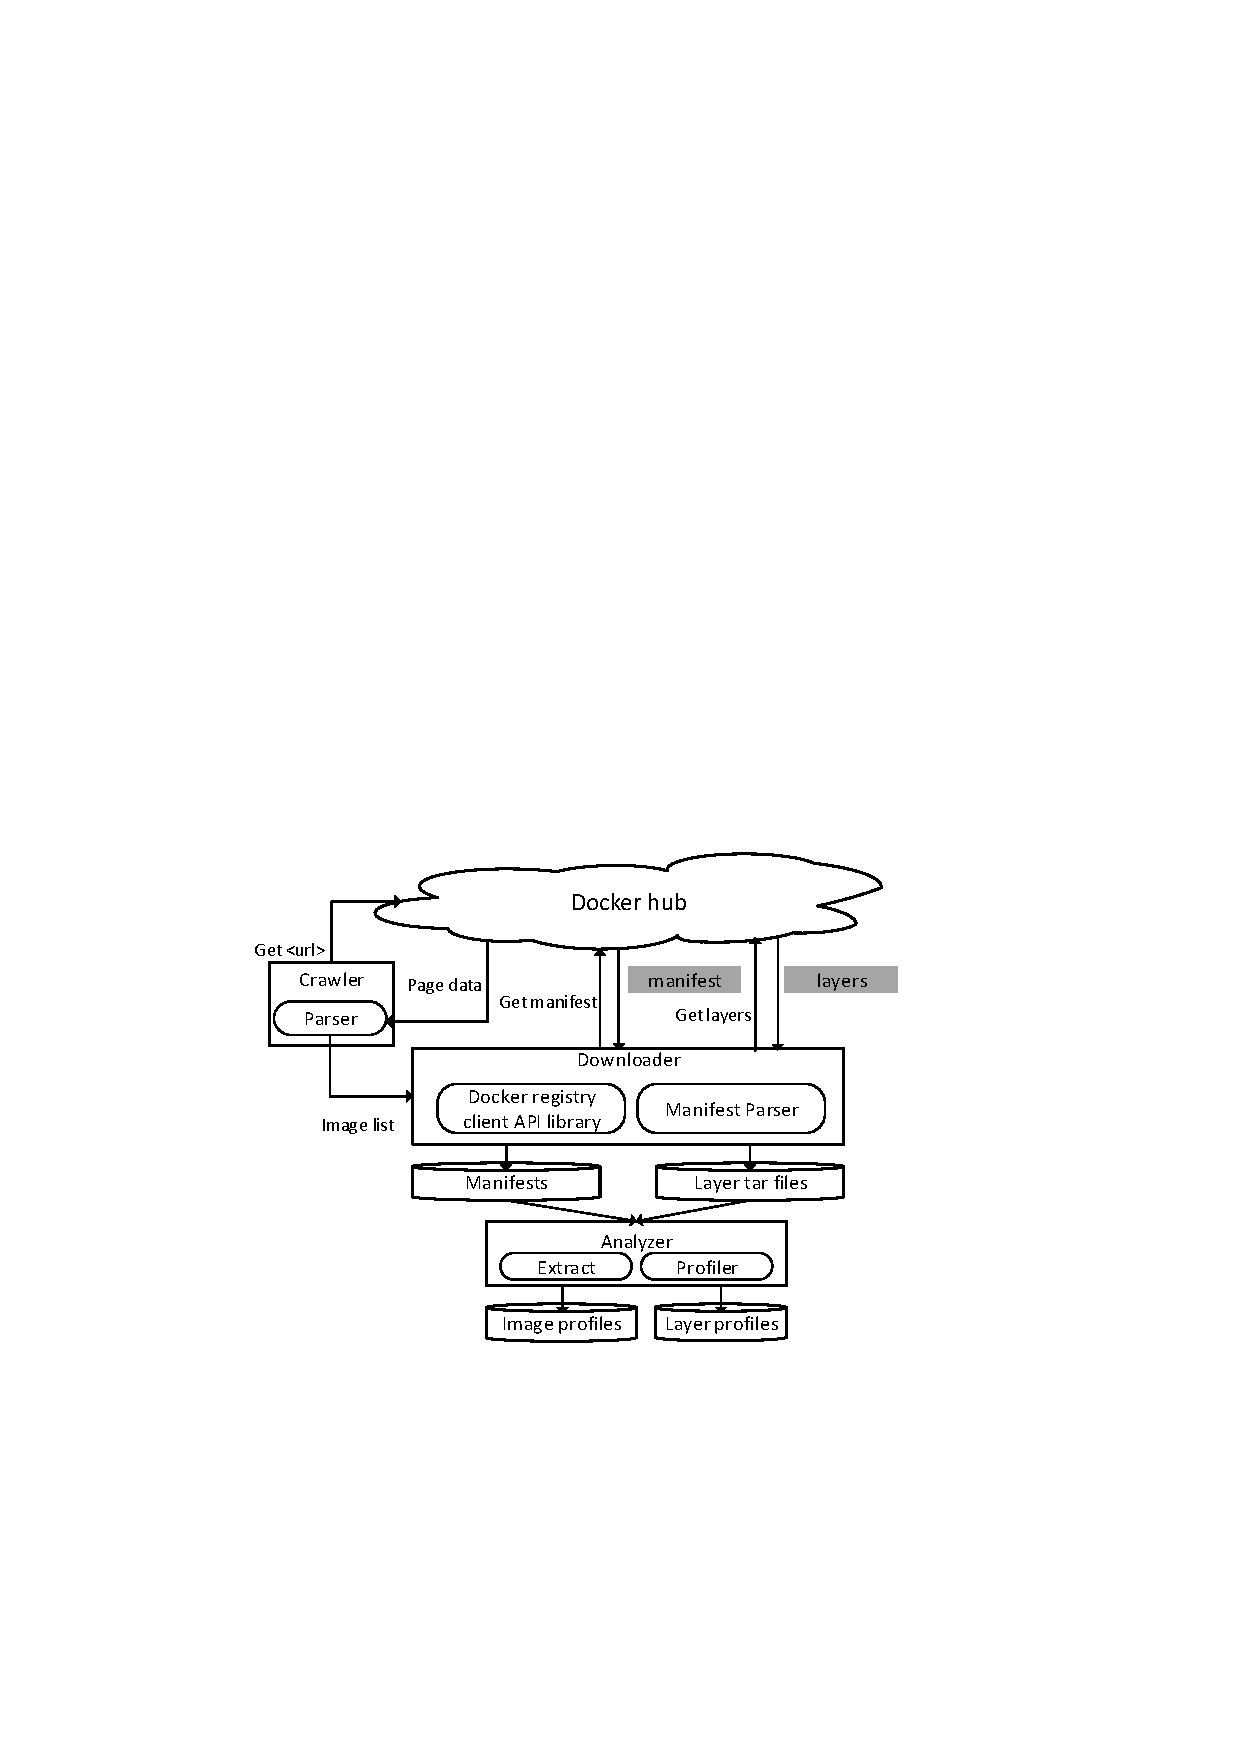
\includegraphics[width=0.5\textwidth]{graphs/fig-downloader-analyzer.pdf}\\
	\caption{Crawler, Downloader, and Analyzer}\label{fig-downloader-analyzer}
\end{figure}

%how container deameon.
%
\subsection{Crawler}
%
To download a particular image, or set of images (i.e., a repository), the
repository name should be provided as mentioned in Section~\ref{XXX}. 
%
A repository is a set of Docker images. The different images in the repository
are labeled with tags.
%
For example, `ubuntu:latest' is the latest version of the Ubuntu image in public
repository Ubuntu.
%
If no tag is provided, Docker engine uses the `:latest' tag as a default. For
example, `docker pull ubuntu' command pulls the `ubuntu:latest' image.
%
\vcomment{Here and in the whole text we need to be very carefull distinguishing names 
of repository and image. Also discussion on image tags is missing, should be in
background section.}
\nancomment{addressed.}
%
Public repositories in Docker registry can be divided into official repositories 
and non-official repositories.
%, where For example, official repository Ubuntu Here is an example of the shared 
%repository official repository Ubuntu and one of its tags. 
%
%A repository is a set of Docker images. A repository can be shared by pushing it to a
%registry server. 
%Public repositories in Docker registry can be divided into official images and non-official 
%images.
%
The amount of official repositories is only ~107 while listing non-official
repositories requires crawling because to the best of our knowledge,
DockerHub (i.e., Docker Hub Registry) doesn't provide an API to list their public
repositories.
%
We therefore created Crawler to crawl Docker Hub website and list public repositories.
%
Docker Hub website provides search engine which indexes public repositories for
users to search for a specific repository or a list of repositories that contains
a certain letter or string. 
%
The name of non-official public repository is comprised
of ``$\langle namespace\rangle/\langle repository name \rangle $",
where~\textit{namespace} is the user name. 
%
In this case, we search for `/' and obtain a list of repositories which contains '/'.
%
In other words, this method lists all the non-official public repositories in Docker Hub.
%
Crawler downloads all the pages which contains `/'.
%
Once web pages are downloaded, it parses the web content and build a list of
non-official repositories. 



Crawler delivered a list of 634,412 repositories on 5/30/2017.
%
However, duplicated repositories exist in the list.
%
After reducing the repeated repositories, our repository list consists of 457,627
distinct repositories. 
%
Note that currently we only downloaded the images with~\textit{latest} tag to
shorten the downloading process. 
%
In the future, we will download all the images with different tags.
%
\vcomment{Explain why, state that it is future work.} 
\nancomment{addressed}
%
\vcomment{I'd comment out discussion on '*'---it has low importance.}
\nancomment{addressed. let's comment it now and see how to deal with this issue}
%Note that the namespace of official images is `\textit{library}'.
%
\subsection{Downloader}

Instead of using Docker (or Docker Engine) to download images, we wrote our own
downloader python script that utilizes Docker Registry API library citeXXX to
simultaneously download~\textbf{original} manifests and layers.
%
\vcomment{Should we mention and cite the library that we used here?}
%
\nancomment{addressed (cited in the following para)}
%
There are several reasons.
%
First, our downloader script runs faster than `\textit{docker pull}' because
Docker Engine performs extra operations other than downloading, such as extracting
tar archive files and converting manifest version. 
%
For example, Docker engine automatically extracting each layer tar archive file
and converts the manifests that are schema version 1 to schema version 2
(starting from Docker engine version 1.10) during downloading process, which
not only consumes considerable time for massive downloading but also affects
our results about manifest version statistics.
%
Second, layer content directories are not visible for some Docker storage
drivers, e.g., devicemapper, which is not feasible to analyze the layer
content. 
%
\vcomment{I think most importantly it is faster because we do not need to
perform extra steps that Docker client performs.}
\nancomment{addressed}
%
Downloader can download multiple images simultaneously and within each image
downloading process, layers are downloaded in parallel.
%
To download the original manifests and layers from Docker Hub, downloader
embeds a library called Docker registry client API citeXXX which only encapsulates
manifest and layer downloading functions in Docker engine without extracting layer
tarball and converting manifest version. 
%
\vcomment{I believe we never explained what is config file. We need to discuss in
in background section.}
\nancomment{addressed}
%
%\subsubsection{Downloading images}




\vcomment{definitely need to merge this subsection with Downloader subsection.
See my comment for the whole section.}
\nancomment{addressed}
%
As shown in Figure~\ref{fig-downloader-analyzer}, downloader first obtains a 
list of public images through crawling Docker Hub.
%
Then, it starts downloading process.
%
It mainly downloads two components: manifest and individual layer files. 



The first step in downloading an image is to fetch the manifest by using the
following url: $GET /v2/\langle name \rangle/manifests/\langle reference \rangle$,
where~\textit{name} parameter refers to
$\langle namespace\rangle/\langle repository name \rangle$.
%
Note that the~\textit{namespace} of official is~\textit{library}.
%
The reference can include a tag or digest.
%
%Note that currently we only downloaded the images with~\textit{latest} tag to shorten
%the downloading process. In the future, we will download all the images with different tags.
%



%
Layers are transferred as compressed tar archive
(i.e.,~\textit{gzip compressed tarball}) in the registry, indexed by digest.
%
\vcomment{What compression is used?}
\nancomment{addressed}
%
As discussed in Section~\ref{xxx}, manifest consist of multiple layer digests.
%
Note that Schema 2 versioned manifest also contains a config file digest.
%
Once the manifest is downloaded, the downloader will then use the digests to
download individual layers (including config file for Schema 2 versioned manifest)
by using the following url: $GET /v2/\langle name \rangle/blobs/\langle digest \rangle$,
where \textit{name} refers to $\langle namespace\rangle/\langle repository name \rangle$
while~\textit{digest} refers to the layer digest or config file digest.

%
\vcomment{I believe different parts of this section belong to different
	earlier parts: some to crawler, some to downloader.}
\nancomment{addressed}
%


The downloading process took roughly 30 days to finish.
%
Overall, we downloaded 51 TB of 355,319 images with 1,792,609 layers as shown
in Table~\ref{XXX}.
%
xxx of images couldn't be downloaded.
%
There are two reasons: first, xxx of images requires authentication.
%
Second, xxx of images don't have tag `:~\textit{latest}'.
%
As we discussed in Section~\ref{xxx}, we only downloaded the images with latest 
version to shorten the downloading process.

\nancomment{2. TODO: add a table discribe:\\
	how many images, duplicate ratio\\
	how many cannot download, (removed, no latest)\\
	how many layers, config, manifest\\
	dataset}

%\subsubsection{Docker image dataset statistics}



%The reason probably is that Docker Hub adjusted websites'order or modified the
%websites because of the increasing of Docker images during our crawling process.
%Our crawler has a unavoidable delay between each HTTP requst and HTTP response. 
%So it couldn't reflect the websites'order or website content changes. Another
%reason is that search engine lists duplicated images 

%Overall, we downloaded XXX image with XXX layers. Table~\ref{XXX} summaries
%the statistics of Docker image dataset we downloaded. Then, we profiled the
%layers, config files, and manifests we downloaded and calculated the statistic
%distribution for different metrics. 

%Some embedded literal typset code might 
%look like the following :
%
%{\tt \small
%\begin{verbatim}
%int wrap_fact(ClientData clientData,
%              Tcl_Interp *interp,
%              int argc, char *argv[]) {
%    int result;
%    int arg0;
%    if (argc != 2) {
%        interp->result = "wrong # args";
%        return TCL_ERROR;
%    }
%    arg0 = atoi(argv[1]);
%    result = fact(arg0);
%    sprintf(interp->result,"%d",result);
%    return TCL_OK;
%}
%\end{verbatim}
%}
%
%Now we're going to cite somebody.  Watch for the cite tag.
%Here it comes~\cite{Chaum1981,Diffie1976}.  The tilde character (\~{})
%in the source means a non-breaking space.  This way, your reference will
%always be attached to the word that preceded it, instead of going to the
%next line.

\begin{table*}
	\centering
	\caption{Dataset summary} \label{tab-dataset-summary}
	\begin{tabular}{c|c|c|c|c|c|c}%p{0.14\textwidth}
		\hline
		% after \\: \hline or \cline{col1-col2} \cline{col3-col4} ...
		Num. of images crawled & Num. of unique images    & Num. of images downloaded  & Num. of layers downloaded \\
		\hline
		634,412                 & 457,627                 & 346,243                    & 1,763,354  \\
		\hline
		Num. of images analyzed & Num. of layers analyzed & Total dataset              &  xxx \\
		\hline
		xxx                     & xxx                     & 51TB                        & xxx  \\
		\hline
	\end{tabular}
\end{table*}

\subsection{Analyzer}

Analyzer analyzes the images we downloaded and creates two kinds of files
for each image: image profile and individual layer profiles.
%
\vcomment{I think we do not need to discuss any metrics above, as you
discuss them below in corresponding subsections.}
\nancomment{addressed}
%
\subsubsection{Layer profile}

As discussed in Section~\ref{xxx}, the layers we downloaded are gzip
compressed tar archive files.
%
To analyze the layer content, analyzer first decompress and extract each
layer tarball to a layer directory.
%
Then, analyzer recursively goes through each subdirectory and obtains
the metadata information for each subdirectory and each file as shown
in figure~\ref{fig-downloader-analyzer}. Each layer profile contains
layer metadata information, such as layer size and file count; and
directory metadata information for each subdirectory, such as directory
depth and directory size; and file metadata information for each file,
such as file size and file type.
%
\vcomment{I'm not sure what figure we want here. I think a table might suffice.}
\nancomment{addressed}
\nancomment{3. TODO: 
	add a fig: discribe all layer metadata, config metadata, and manifest metadata structure} 

\nancomment{4. TODO: 
	add a table\\
	layer tarball format statistics, tar, compressed, non compressed\\
	config statistics, txt, json\\
	manifest statistics, txt, json}





\subsubsection{Image Profile}

As shown in figure~\ref{fig-downloader-analyzer}, Analyzer parses the manifest
and obtains the configuration information such as os, architecture etc..
%
Note that manifest Schema version 2 stores configuration information in a
config file as discussed in Section~\ref{xxx}.
%
As shown in table~\ref{xxx}, xxx of manifests are Schema version 2 while the
rest are Schema version 1. 
%
Once individual layers are analyzed, analyzer can build the whole image
profile by including pointers to its layer profiles as shown in
figure~\ref{xxx}. Each image profile includes image metadata information,
such as image pull count and layer count, and image configuration
information, such as os version and architecture; While layer profile
contains layer metadata information, such as layer size and file count;
and directory metadata information for each subdirectory, such as directory
depth and directory size; and file metadata information for each file, such
as file size and file type.
%
Table~\ref{xxx} summaries the layer archive file, config file, and manifest
statistics.


\vcomment{This section (and some other places) contain a lot of ``etc.''. The
general rul of thumb never to ue etc. in a scientific paper. Instead,
say: "e.g.,", or "for example," or "for instance"}
\nancomment{addressed}
%\subsubsection{Config profile}

